\RequirePackage{fixltx2e} %This package in CTeX is not compatible with revtex4-1
\documentclass[aps,pre,12pt,preprint,onecolumn,showpacs,showkeys]{revtex4-1}
\usepackage{ctex}
\usepackage{mathtools}
\usepackage{multirow}
\usepackage{setspace,dcolumn}
\usepackage{hyperref}
\usepackage{graphicx,psfrag,epsfig}
\usepackage[font=small,format=plain,labelfont=bf,textfont=it,justification=centering,singlelinecheck=false]{caption}
\usepackage{amsmath,amsfonts,amssymb,amsthm,bm,upgreek}
\usepackage{geometry}
\usepackage[mathscr]{eucal}
\usepackage{caption}
\usepackage{subcaption}
\hypersetup{colorlinks=true}
\geometry{top=2.54cm,bottom=2.54cm,left=3cm,right=3cm}
\renewcommand\appendixname{附录}
\renewcommand\abstractname{}%摘要
\renewcommand\tablename{表}
\renewcommand\figurename{图}
\makeatletter
\def\@pacs@name{\songti\zihao{-4}{\bf PACS码:}}
\def\@keys@name{\songti\zihao{-4}{\bf 关键词:}}
\def\Dated@name{日期:}
\def\Received@name{\zihao{-5}{接收} }
\def\Revised@name{\zihao{-5}{修订} }
\def\Accepted@name{\zihao{-5}{采纳} }
\def\Published@name{\zihao{-5}{发表} }
\makeatother
\linespread{1.3}
\renewcommand{\labelenumi}{\alph{enumi}.}
\leftmargini=20mm
\def \d {\mathrm d}
\def \cs {\frac{\d \sigma}{\d \Omega}(\theta)}
\def \csref {\frac{\d \sigma}{\d \Omega}(\theta_0)}
\def \Cs {^{137}\mathrm{Cs}}
\def \Co{^{60}\mathrm{Co}}
\def \degree {^\circ}
\def \V {\mathrm{V}}

\begin{document}
\title{\bf\heiti\zihao{3}扫描隧穿显微镜\vspace{15mm}}
\author{\fangsong\zihao{4}邵智轩\vspace{2mm}}
\affiliation{\songti\zihao{-4}学号:1400012141\vspace{2mm}}
\date{\today}
%\pacs{02.10.Yn, 33.15.Vb, 98.52.Cf, 78.47.dc}
\keywords{量子隧穿,恒流模式,减震,针尖,偏置电压,压电陶瓷,石墨}
\email{shaozhixuansh@pku.edu.cn; (86)13381350619}

\begin{abstract}
\vspace{10mm}
\begin{spacing}{1.5}
\songti\zihao{-4}
扫描隧道显微镜(scanning tunneling microscope,缩写为STM)是一种利用量子隧穿效应的非光学显微镜。本实验的目的是学习和掌握扫描隧穿显微镜的原理和结构,观测量子力学中的隧穿效应,学习扫描隧穿显微镜的操作和调试过程,并用STM来观测样品的表面形貌、得到原子分辨的图像。
\end{spacing}
\end{abstract}
\maketitle
\songti\zihao{-4}

\section{引言}
扫描隧道显微镜是一种利用量子隧穿效应探测物质表面结构的仪器。它于1981年由格尔德·宾宁及海因里希·罗雷尔在IBM位于瑞士苏黎世的苏黎世实验室发明,两位发明者因此与电子显微镜的发明者恩斯特·鲁斯卡分享了1986年诺贝尔物理学奖。

扫描隧道显微镜技术是扫描探针显微术的一种,基于对探针和表面之间的隧穿电流大小的探测,可以观察表面上单原子级别的起伏。此外,扫描隧道显微镜在低温下可以利用探针尖端精确操纵单个分子或原子,因此它不仅是重要的微纳尺度测量工具,又是颇具潜力的微纳加工工具。
 
\section{实验原理}
对于能量为$E$的粒子,不同于经典理论,在量子力学中,在势能$V(r)>E$的区域,薛定谔方程
\begin{equation}
\left[ -\frac{\hbar^2}{2m} \nabla^2 +V(r)\right] \phi(r)=E \phi(r)
\end{equation}
的解$|\phi|^2>0$(近似指数衰减),即一个例子要穿透一个$V(r)>E$的势垒的几率是非零的。这就是STM最基本的原理。

%作为局域探测手段,必须有四个技术要素:
%\begin{enumerate}
%\item 与距离有强烈依赖关系的相互作用
%\item 局域探针
%\item 探针和样品之间极近的距离
%\item 在零点几个纳米的有效相互作用范围内精确地保持探针和样品位置的相对稳定
%\end{enumerate}
%前三个要素决定仪器分辨率的大小,第四个要素则是得到理想分辨率的保证。

STM的核心是一个能在表面上扫描并与样品间有一定偏置电压的针尖,当针尖与样品十分接近时,它们之间的势垒变得很薄,在实验中就能观察到隧穿电流。通过记录针尖与样品间的隧穿电流间的变化就可以得到样品表面形貌的信息。

隧穿电流$I$与两电极之间的距离$S$的关系为:
\begin{equation}
I\propto B\exp(-KS)
\end{equation}
其中$K=\sqrt{2m(V-E)}/\hbar$,$m$为自由电子的质量,B为与样品的偏压$V_b$有关的系数。STM的针尖和样品之间构成势垒的间隙$S\approx 1 \mathrm{nm}$。可以粗略地说,$S$每改变0.1 nm,隧穿电流就会改变一个量级,从而隧穿电流几乎总是集中在间隔最小的区域。

根据隧穿电流的这一特性,在STM中把针尖装在压电陶瓷构成的三维扫描架上,通过改变加在陶瓷上的电压来控制针尖位置,在针尖和样品之间加上偏压$V_b$以产生隧穿电流,再把隧穿电流送回到电子学控制单元来控制加在$z$向陶瓷上的电压。工作时,在$x$、$y$向陶瓷上施加扫描电压,针尖便在表面上扫描。扫描过程中表面形貌起伏引起的电流的任何变化都会被反馈到$z$向陶瓷,使针尖能够跟踪表面的起伏,以保持隧穿电流的恒定。记录针尖高度作为横向位置的函数$z(x,y)$(即$z$向压电陶瓷的电压)得到表面形貌的图像。这便是STM最常用的\textbf{恒流模式},如图\ref{fig:mode}中的(a)所示。
\begin{figure}[h]
\centering
\includegraphics[width=60mm]{mode}
\caption{\label{fig:mode}%
STM的两种工作模式}
\end{figure}

此外STM还有恒定高度的工作模式,如图\ref{fig:mode}中的(b)所示。此时控制$z$向陶瓷的反馈回路虽然仍在工作,但是反应速度很慢,以致不能反映表面的细节,只能跟踪表面的大起伏。这样,在扫描中针尖基本上停留在同样的高度,而通过记录隧穿电流的大小得到表面的信息。一般高速STM便是在此模式下工作,但由于在扫描中针尖高度几乎不变,在遇到起伏较大的表面(如起伏超过针尖样品间距0.5 - 1 nm 的表面),针尖容易被撞坏。因此这种模式只适合测量小范围、小起伏表面。

\section{实验装置}
STM简要的工作原理如图\ref{fig:equip}所示。
\begin{figure}[h]
\centering
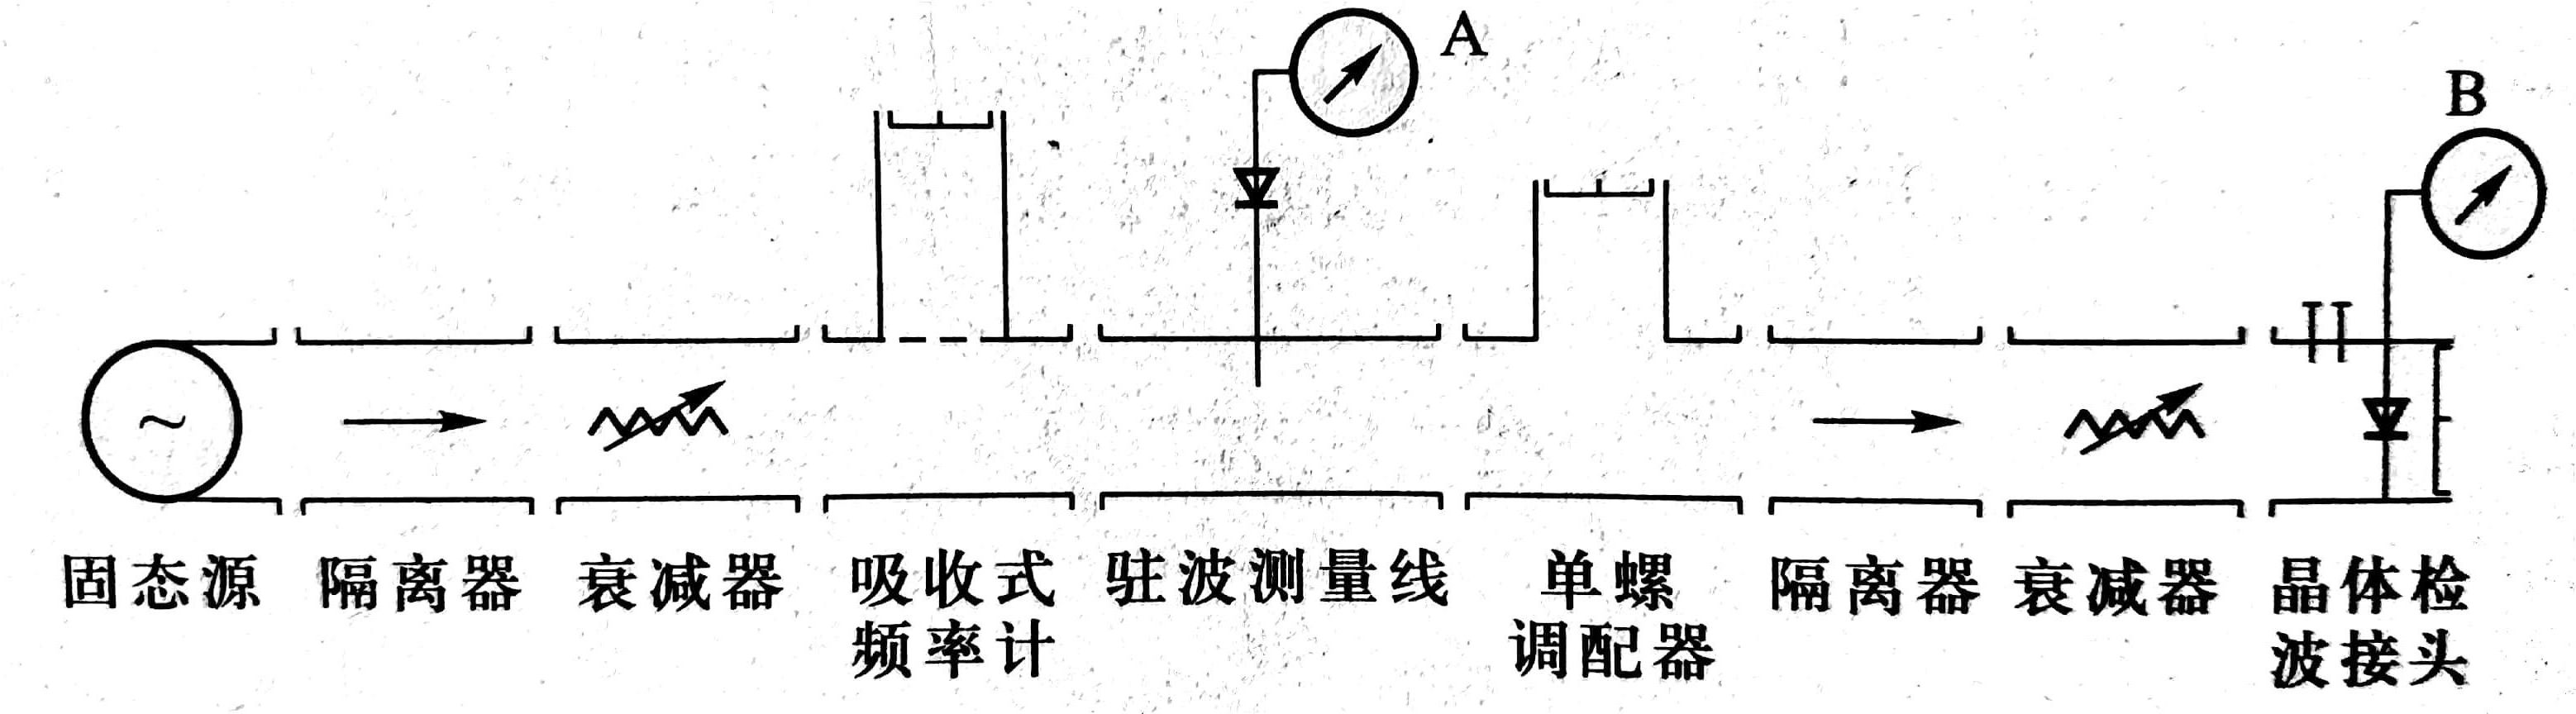
\includegraphics[width=80mm]{equip}
\caption{\label{fig:equip}%
STM工作原理示意图}
\end{figure}

STM 由减震系统、粗逼近、扫描架和电子学控制单元构成。

减震系统由挂在系统内的四根长弹簧和STM 底盘上的氟橡胶条构成:其中弹簧的共振频率尽可能小,以隔离低频振动,而氟橡胶条可以减少多种频率的震动。

粗逼近系统为通过计算机控制的步进马达带动的蜗轮蜗杆变速装置,它由传递系数很低的高精度蜗轮蜗杆减速箱带动一根坚固的丝杠向前推动样品。电流探测回路测量针尖和样品间的隧穿电流,一旦探测到非零的隧道电流,计算机控制马达便立即止步,并发出警报。这种设计的粗调节范围约为1cm,步幅为50nm/步,步进速度可变,保证了样品自动、快速并且安全的实现粗逼近。

扫描架由两对陶瓷杆和一根陶瓷管支撑着的牢固结构组成。两对陶瓷杆的材料、压电系数和长度是一样的,因此当$x$,$y$电压分别加在反极性并联的每对陶瓷杆上时,它们形成的互补结构可以有效地减小热漂移。管状的$z$ 向陶瓷具有较大的压电系数和较高的固有频率,使扫描架可以具有较大的动态范围。

另外,STM 由一台PC 机和电子学单元控制,分为工作电源和隧穿电流反馈控制与信号采集两大部分。前一部分提供X,Y扫描电压和Z 高压,后一部分则包括样品偏压、马达驱动、隧穿电流的控制和信号采集的模数转换等。
\begin{figure}[h]
\centering
\includegraphics[width=80mm]{Graphite.jpg}
\caption{\label{fig:structure}%
石墨的的晶体结构}
\end{figure}

实验样品为高定向热解石墨(HOPG)。石墨是碳的一种同素异形体,其晶体结构如图\ref{fig:structure}所示。它具有层状的平面结构,每层中碳原子都排列呈蜂窝状晶体结构。层内每个碳原子的周边以共价键连接另外三个碳原子,排列方式呈蜂巢式的正六边形。

\section{实验过程与结果}
针尖由电化学腐蚀的方法制备。由于时间关系和操作难度,本实验开始前探测用的针尖已制备好。

\subsection{粗逼近}
设置隧穿电流初始值为1nA,样品偏压初始值为1000mV。根据菜单提示进行粗逼近,进入隧穿状态时时,计算机会发出蜂鸣报警并自动停止进针。手动单步进针使$z$方向上电压示数略小于100mV后,再退针20 步,使得步进马达与针尖脱耦,以减小步进马达振动对系统的影响。实验中针尖高度也会缓慢漂移,即$z$向电压会随时间缓慢升高,当$z$向电压增大至靠近200 mV时,需要重复上述粗逼近的操作使其回到100mV 左右,以保持隧穿状态。

\subsection{得到石墨的原子分辨像}
先大范围扫描,尽量找一块平整的区域。初始的扫描范围为$200\mathrm{V} \times200\mathrm{V}$,原点$X_0=0\mathrm{V}$,$Y_0=0\mathrm{V}$。扫描时间近似与扫描范围成线性关系,即范围为200 V 时扫描时间为2000 ms;范围为 2 V 时扫描时间为400 ms,并可在上下$\pm 50\%$的范围内调节。点击开始扫描后,调节offest使扫描波形完整,并在允许的范围内尽量调高信号增益倍数以增强对比度。扫完完整的图像后,找一块平整的区域,跟踪该区域,将原点调到该区域的左下角,并适当加大放大倍数(缩小扫描范围)。

\begin{figure}[h]
\centering
	\begin{subfigure}[t]{60mm}
		\centering
		\includegraphics[width=60mm]{1}
		\caption{$200\V \times 200\V$}\label{fig:200times200}		
	\end{subfigure}
	\quad
	\begin{subfigure}[t]{60mm}
		\centering
		\includegraphics[width=60mm]{2}
		\caption{$100\V \times 100\V$}\label{fig:100times100}
	\end{subfigure}
	\caption{大范围扫描的HOPG原子分辨像,红框标出下一步的扫描区域}\label{fig:broad}
\end{figure}

大范围扫描下得到的STM 成像如图\ref{fig:broad}所示,图中红框标出下一步的扫描区域。
\begin{figure}[h]
\centering
	\begin{subfigure}[t]{60mm}
		\centering
		\includegraphics[width=60mm]{4}
		\caption{$4\V \times 4\V$}\label{fig:4times4}		
	\end{subfigure}
	\quad
	\begin{subfigure}[t]{60mm}
		\centering
		\includegraphics[width=60mm]{final}
		\caption{$2\V \times 2\V$,可以清晰地看到有心六角密排}\label{fig:2times2}
	\end{subfigure}
	\caption{小范围扫描的HOPG原子分辨像}\label{fig:small}
\end{figure}

逐渐缩小扫描范围(放大倍数增加),摸索、调整增益和扫描时间等参数,逐渐使像变得清晰。小范围扫描下的成像如图\ref{fig:small}所示,在图\ref{fig:2times2}中可以清晰地看出有心六角密排结构(将在思考题\ref{sec:q}中给出讨论)。

\subsection{标定$x$、$y$陶瓷的压电系数}
利用已知的HOPG原子间距 0.246 nm 来计算像的实际尺寸,以此标定$x$、$y$陶瓷的压电系数。
\begin{figure}[h]
\centering
\includegraphics[width=80mm]{final_1}
\caption{\label{fig:measure}%
估算$x$、$y$陶瓷的压电系数。图中取了4个点A (72,45),B (122,197),C (78,166),D (232,38)。}
\end{figure}

在图\ref{fig:measure}中,
$$\overrightarrow{A B}=(50,152),\quad |AB|=160.0, \quad\text{横跨7个原子}$$
$$\overrightarrow{CD}=(154,-128), \quad |CD|=200.2, \quad\text{横跨8个原子}$$
$|AB|/|CD|<7/8$,图中六边形并非严格的正六边形,$x$方向与$y$方向的比例尺是不同的。设图中的向量$(x,y)$对应真实的向量$k(x,\beta y)$,$k$为$x$方向的比例尺,$k\beta$为$y$方向的比例尺。记$\overrightarrow{AB}=(x_1,y_1),\quad\overrightarrow{CD}=(x_2,y_2)$,利用$\overrightarrow{AB}$与$\overrightarrow{CD}$实际的夹角应为$120\degree$这一信息,我们可以得到计算得到
$$-\frac{1}{2}=\cos 120\degree=\frac{x_1 x_2 +\beta^2 y_1 y_2}{\sqrt{x_1^2+\beta^2 y_1^2}\sqrt{x_2^2+\beta^2 y_2^2}}$$

带入$(x_1,y_1)$,$(x_2,y_2)$得到$\beta^2=1.4672$

再利用真实的C与D间的距离求得比例尺$k$
$$k\sqrt{x_2^2+\beta^2 y_2^2}=8\times0.246\mathrm{nm} \quad\text{解得}\quad k=9.06\times 10^{-3} \mathrm{nm}$$
从而图像中$x$和$y$方向的实际长度:
$$l_x=k\times 256=2.32 \mathrm{nm}$$
$$l_y=\beta l_x=2.81 \mathrm{nm}$$
故$x$和$y$方向的陶瓷压电系数:
$$\text{$x$方向:} \frac{2.32 \mathrm{nm}}{2.0\V}=1.16 \mathrm{nm/V}$$
$$\text{$y$方向:} \frac{2.81 \mathrm{nm}}{2.0\V}=1.41 \mathrm{nm/V}$$

\section{总结}
本实验通过调整样品偏压,扫描时间,扫描范围等参数,减小热漂移,提高成像清晰度,最终获得较为清晰的高定向热解石墨 (HOPG )的原子分辨像,成六角密排。并通过 HOPG 原子分辨像中已知的原子之间距离标定了 X,Y 方向的压电陶瓷系数,分别为1.16 nm/V 和 1.41 nm/V。

\section{致谢}
感谢指导老师季航,以及我的合作者李少楠。
\begin{thebibliography}{}
\bibitem{Book} 吴思诚, 荀坤 2015 近代物理实验(第四版)(北京:高等教育出版社).
\bibitem{Book} 赵凯华, 罗蔚茵 2001 新概念物理教程—量子物理 (北京:高等教育出版社)
\end{thebibliography}
\clearpage
\appendix
\section{实验报告思考题}\label{sec:q}
HOPG的原子排列为六角密排(无心的),为什么我们在实验中看到的HOPG的原子分辨像是有心的六角密排?
\begin{figure}[h]
\centering
\includegraphics[width=80mm]{10}
\caption{\label{fig:demon}%
HOPG晶体结构}
\end{figure}

如图\ref{fig:demon}所示,HOPG每一层原子都成无心六角密排结构,且每一层原子都可分为A,B 两种。A 原子与下层原子重叠,B 原子位于下层原子六角密排结构的中心,受下层原子的吸引较强而位置相对A 原子偏下。故STM 扫描像中A 原子呈一亮斑,而B 原子较 A原子会更暗,易被忽略。若忽略B 原子只看A 原子的排列结构,确实呈现有心六角密排,正如图\ref{fig:2times2}中那样。


\end{document}
